\chapter{Proposed System}
\section{Overview}
Last chapter we discuss the audio data hiding method, which plays an important role in our system. It is the core that other parts of our system revolve around. However, without a logic system to flow data, the core has nothing to process and output. Recall that our project is about an streaming system that integrate watermark embedding before the streaming process. The output of our endpoint are audio data that are watermarked. Therefore, there are many processes that we need to take care, each will interact with each other to work together as a whole system.

Our system comprises of the server and client application. On the client side, we have 2 things to keep in mind: Audio watermark decoding and audio playback. Very straightforward, the audio data is decoded by a watermark decoding process and then sent to the playback component. If the audio fragment contains a embedded watermark, display the information when the sound is played. On the other hand, the server requires more considerations for its complexity. There are many things happening at 1 point of time on the server. While constantly waiting for the desired information to embed, we also do audio processing and produce audio data. That very audio data is sent to another module responsible for streaming to clients. Not to mention managing clients connection and authentication should not be taken lightly. Therefore, ideally, our server application contains smaller modules that independently contribute to the system as a whole, working together in harmony without stepping on each others toes. First, if an embedding information is received from the input, this module sends signal to the audio processing to do embedding. Afterwards, the audio module itself continues the flow by sending the embedded data to the streaming service and broadcast to clients. Moreover, all of those mentioned procedures independently execute on their own. For example, the streaming service continually sends data to clients and does not care if the data contains embedded information or not. 

We need an audio watermark process, obviously. This part takes audio data and a watermark string as input. It then employ the audio watermark embedding method we proposed last chapter and produce watermarked audio data as output. Our logic system help send data to this process and take its output to other processes. Hence, other processes as watermark input and streaming process is needed. The input process runs continuously and wait for watermark input, then it send the information to audio watermark process. After the watermarking process done embedding, it send watermarked audio data to the streaming process. The streaming process send audio data to clients and then wait for the next audio data to come. These processes run on its own, independently and send its result to other processes. Overall, we have a system illustrated in Figure \ref{fig:Server}. It’s also worth noting that we have our process running independently and interact with each other  to alter the flow of the program execution. In order to realize that, we need tools to employ such concept as concurrency. After identify the needed features of our server application, we realize that we need a framework to build those small modules and glue them together. To realize this idea, we came up with a system design that rely on the field of communicating sequential processes. Specifically, concurrency is our goal. Concurrency is a way to divide the existing big problem into smaller parts that are independent. This is where we take advantage of Golang and its support for concurrency.

\subsection{Server setup}

Seeing how complex the idea of concurrency is, we shift to finding a mechanism to realize this without implement it ourselves. Apparently, it is best that we apply the assistance from a specialized programing language. Partly, to accomplish our original idea, system designing is put at the highest priority, but it would be so much easier if we utilize on a programming language and its intrinsic properties that help us implement this more effectively. After much discussion, we bring another result of our research engineering process into the project as we choose Golang as the programming language for the server application. Golang is a relatively new programming language invented by Google with focus on concurrency. Golang features built-in properties that support concurrency. As mentioned earlier, we modularize our system into smaller parts that work independently. At this point, we apply the goroutine concept from golang to help achieve this. Goroutines are lightweight threads allocated for an instance of a function to execute independently. In our case, we have 4 goroutines that continually running. Golang also introduces channel, as a mean for goroutines to signal each other. For instance, if the input goroutine receive an actual input, it sends the input data through the channel that connects to the audio processing goroutine. Consequently, this function changes its way of processing audio data, switching to do audio embedding with the input data received. Otherwise, the audio processing module would only extract audio data, no watermarking is involed. The streaming goroutine does not care how the audio process deals with data, it only takes audio data that the audio module sends through a channel, and stream to clients. Meanwhile, if there are any new client connect to the streaming point, the client manager goroutine persist the connection for further data streaming. All of those goroutines works independently and signal each other for data. We call this share memory by communicating, not communicate by sharing memory. This is the main compass of the Golang programming language.

\begin{figure}[bt]
\center
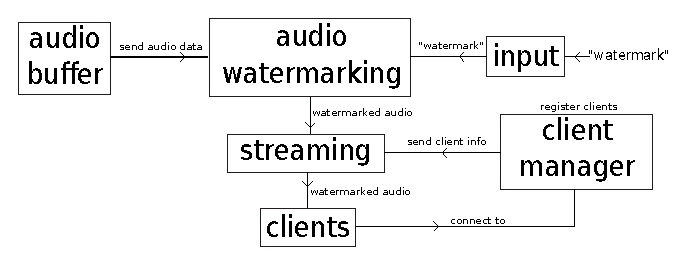
\includegraphics[width=.9\columnwidth]{system.eps}
\caption{Our server flow chart}
\label{fig:Server}
\end{figure}

With the strong support from Golang, it becomes less painful when implementing the design architecture. However, what Golang does is simply provide us a tool to better systemizing. It is important that we have a solid ground of system design that Golang can relies on and do what it is best at. At the front line, we have the audio processing sequentially scans through the audio file and extract a frame of audio samples with fixed length. This frame is pushed into the queue waiting to be sent to the steaming module, where we also have a queue. The reason why we apply queues to handle data is congestion preventation while also assure a decent amount of spare space for unusually long watermarking information. Specifically, when a big input is received and the current audio frame is not enough for embedding, we should not wait for the next frame because it would increase the overhead cost for the system. What best is take the remaining frames in the queue and fill them up with embedding information. On the other hand, the streaming module also needs a queue to make sure the situation of data starve will not occur. Otherwise, without a queue, if the audio embedding takes too much time to complete, the client have to wait for data to produce sound to listeners, and that is not good at all.

\subsection{Client setup}
At the client, we would like to keep it as simple as possible, since this is where the user experience our product and it's wise to keep the implementation straightforward and less error prone. Therefore, we decided to choose the simple popular frontend web framework AngularJS\cite{angular}. This piece of technology require very little effort to get up and running. However, we still face some engineering obstacles. First, it is very important what technology we choose to establish a connection betweeen the server and client. We would like it to be a stream of continuous data, without having to re-create the connection each time new data is to be sent. There are many solution for our streaming, we can rely on a third party program like Gstreamer\cite{gstreamer} to do the streaming for us, or utilize a builtin feature of our very mechanism of connect to the internet: browser. 

We then do a small research and sketch out some strengths and weakness of the two ways. For Gstreamer, it would lift a burden for us doing streaming on it own, we only need to feed data for it and everything is set. Unfortunately, there is a high chance we can not integrate it into our existing system. Since streaming involves both the server and client and it less likely to combine many technologies together. On the other hand, if we invest resources into researching an intrinsic streaming feature of our existing system, which are Golang and AngularJS, we then can be sure about compatibility of our system. Afterward, we proceed to look for a suitable means for our streaming process. We found out that both Golang and AngularJs support websocket. Moreover, it is also a simple solution that we can pickup very quickly.

In the end, we have a client set up illustrated in Figure \ref{fig:Client}

\begin{figure}[bt]
\center
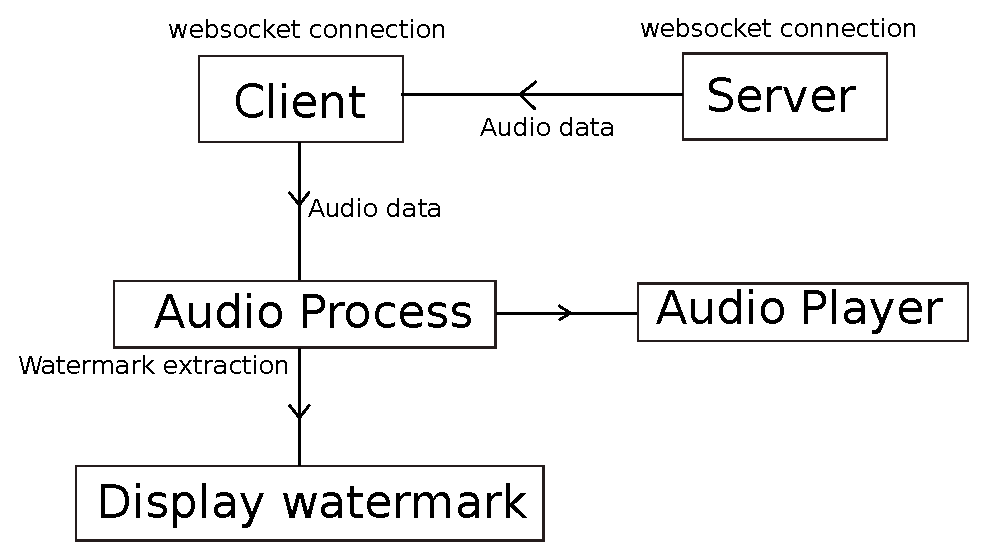
\includegraphics[width=.9\columnwidth]{client.eps}
\caption{Our client flow chart}
\label{fig:Client}
\end{figure}

\section{Proposed System in Details}
\subsection{Watermark Input Process}
Watermark input process is the first stone of our system, it acts as a receiver, waiting for input and send to other processes. Specifically, we spawn a Goroutine to execute on its own. When watermark is received, this process takes in characters as input and feed to a predefined channel. This channel associates with other processes and send watermark input to them. The input process is briefly illustrated in Fig \ref{fig:InputProcess}.

We would like the process to sleep for 5 seconds to avoid input abuse. Otherwise, if there are too many watermark strings to embed, it would be difficult to track result. We recommend that we put all our watermark strings into a big string to do embedding for only once.

\begin{lstlisting}
// Watermark Input Process
func (ms *MarkStream) Input() {
	reader := bufio.NewReader(os.Stdin)
	for {
		log.Printf("Input your embedding string: ")
		text, _ := reader.ReadString('\n')
		ms.userInputChan <- text
		log.Println("Embedding...")
		time.Sleep(5 * time.Second)
	}
}
\end{lstlisting}

\begin{figure}[bt]
\center
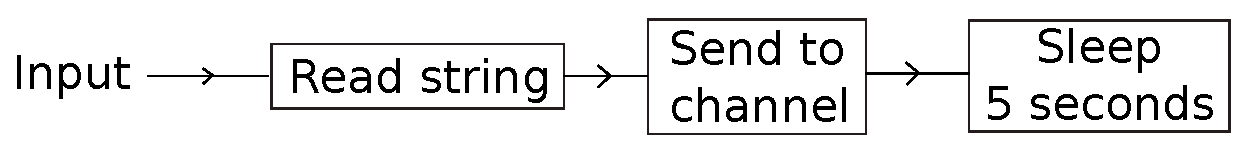
\includegraphics[width=.9\columnwidth]{inputprocess.eps}
\caption{Watermark receiver}
\label{fig:InputProcess}
\end{figure}

\subsection{Audio Watermarking Process}
\begin{figure}[bt]
\center
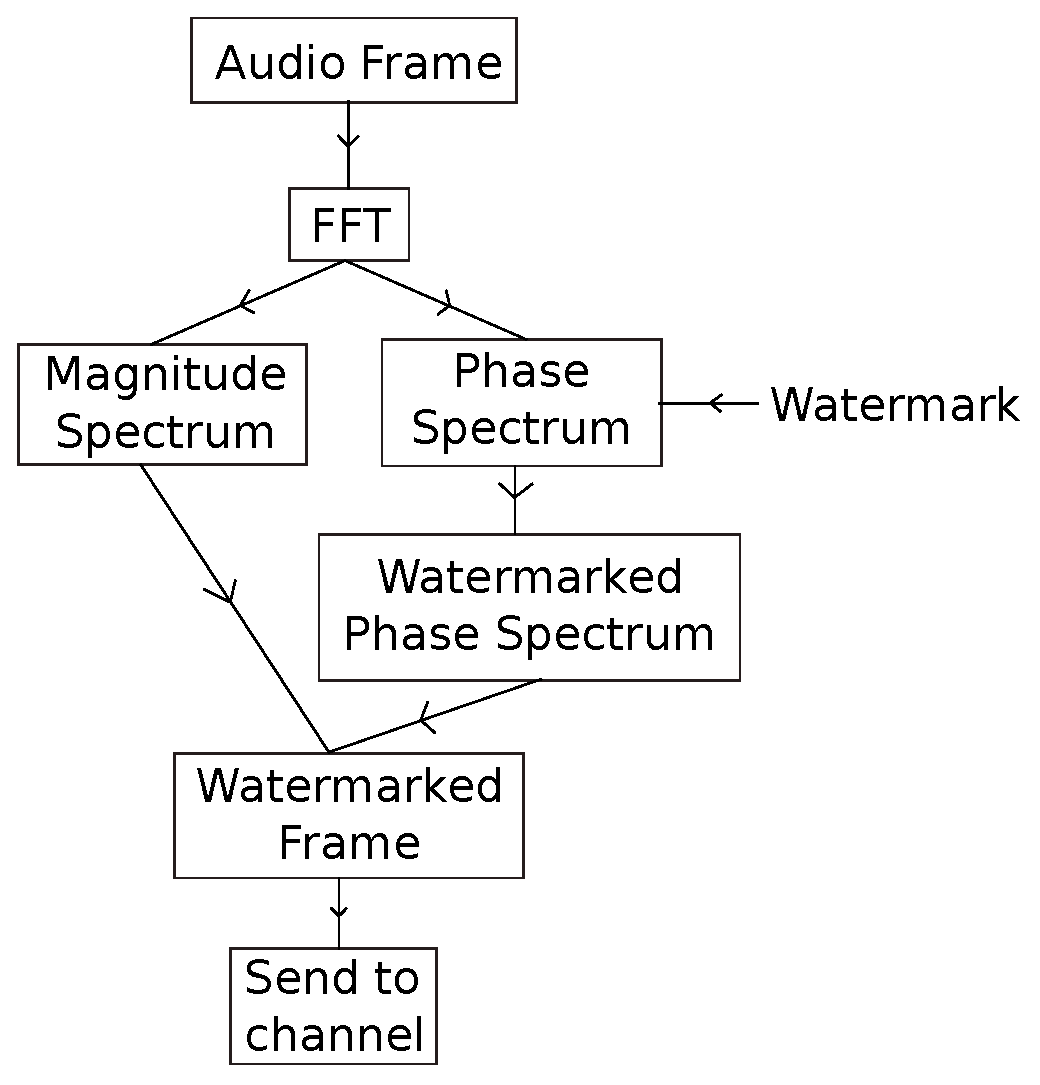
\includegraphics[width=.9\columnwidth]{watermarkingprocess.eps}
\caption{Audio watermarking process}
\label{fig:WatermarkingProcess}
\end{figure}
The core of our system lies at the audio watermarking processing. It should be noted that producing a good quality, low error rate, embedded audio file is not something could be taken by granted. Instead, it is a process of trade-offs that we must examine carefully. At the time of this research, there are many watermarking methods available. Some methods remove the least significant bits to make space for the watermark (LSB), or shape the watermark according to the human auditory system (HAS). Other methods use the simultaneous masking characteristics of HAS or relative insensitivity of phase change to embed inaudible watermarks. Phase coding is used because since controlled phase alteration results in inaudible change in sound to HAS. On the other hand, to improve robustness, quantization index modulation (QIM) is employed and has shown promising results with several audio watermarking methods. We would like to combine the greate result of inaudibility and robustness together to produce audio that not only has good quality but also solid against several attacks in robustness. The idea is to transform the original time domain audio data into frequency domain by Fourier transform (FFT is used). Result of the transformation is the magnitude and phase components of the frequencies bins. QIM is used here to embedd a bit, either 0 or 1, into the original phase. Depends on the magnitude component of the bin, we decide how much change we apply to the phase component. The result is new phase components that are slightly different compared to the original ones. Finally, using the Inverse Fourier tranform, we remake the audio data by combining the magnitude components and the new phase components. The final outcome is new audio data that are embedded. This method is called dynamic phase coding. It takes one step further than the tradition phase coding, where we only use one fixed amount of modification to adjust the phase. Since the audio features contains a lot of different frequencies, using just one standard can not cover all the possible values and end up only effective for a certain range of frequencies. Other ranges would result in either bad quality audio or highly error prone watermarking. 

Audio watermarking is the primary part of our system. It process audio data while also wait for watermark input and do embedding. If there is no input is received, ordinary audio data is produced. All of those output is sent to the streaming Goroutine to handle.

It’s important to know that audio file is made of mere integers, which is called samples. For our project, we represent an integer by 16 bits \(=2\) bytes. This process continuously waits for audio data to come  and perform necessary actions to do audio processing. Specifically, for each 500ms, it receives a slice of the data of length 22050 samples, which means \(22050*2=44100=44.1kB\). For the sake of our project development, we simply create another Goroutine responsible for sending out audio data. In reality, we would have a stream of audio of our own. The audio watermarking process is illustrated in \ref{fig:WatermarkingProcess}

Recall that the output of our server is a stream of audio data, nothing else. Therefore, there is a technical challenge about how to notify client when a watermark is embedded. We studied that the cost of audio embedding is not too much and we can do it without any overhead burden in terms of memory assumption and execution time. In fact, embedding an audio frame with framelength of \(22050\) only costs us \(0.05\) second. Therefore, we decided to embedd a notifying character to solve the problem of watermarking synchronization. There are two cases of flow control for this process.
\subsubsection*{There is no input received}
In this case, our embedding string is only a chacter \('0'\), which costs us \(8*5=40\) samples to embed, where 8 is the number of bits for character \('0'\) and 5 is how many times we repeat 1 bit to ensure embedding correctness. Then, when the client receive our audio data, they will employ watermark extraction and understand that there are no input embedded in this particular audio frame.
\subsubsection*{There is input received from the channel of the input process}
In this case, our embedding string is \('1' + input\). The steps of execution are the same and produce a watermarked audio frame. If the input to embed is too long and exceed the length of maximum samples we can embedd, which is \(800\), then we continue the embedding in the next audio frame. It's very crucial that we only do audio processing on the first \(800\) samples of the audio frame. Otherwise, we probably produce a low quality audio data and hightly error prone for watermark extraction.

\subsection{Client Managers and Audio Streaming Process}
We also have a client manager to store client's connections for streaming purpose. In engineering terms, we open a websocket endpoint waiting for clients to connect. Each time a client comes in, we spawn a temporary Goroutine reponsible for that particular client. In this specific Goroutine, we create a unique identity for this new client and save its connection in an array for further use. Then, this Goroutine ends asynchronously, only the array of client connection is preserved.

In this process, when we receive audio frame from the watermark embedding process, we iterate through the list of clients and send audio data to them. Another note is about the format for streaming over the Internet. The result of the watermarking process is an array of \(float64\) numbers. If we choose to broadcast this type of data over the Internet, the cost would be huge and potentially cause incompleted data. Therefore, we scale down the output to only \(int16\) type, which does not affect the accuracy of data much. By this way, we broadcast our audio data over the Internet with a minmized cost while still ensure its quality.

The technolgy we use to streaming is websocket\cite{websocket}. WebSocket is a protocol providing full-duplex communication channels over a single TCP connection. It is designed to be implemented in web browsers and web servers, but it can be used by any client or server application. The WebSocket Protocol is an independent TCP-based protocol. Its only relationship to HTTP is that its handshake is interpreted by HTTP servers as an Upgrade request. The WebSocket protocol makes more interaction between a browser and a web server possible, facilitating the real-time data transfer from and to the server. This is made possible by providing a standardized way for the server to send content to the browser without being solicited by the client, and allowing for messages to be passed back and forth while keeping the connection open. In this way, a two-way (bi-directional) ongoing conversation can take place between a browser and the server

\begin{lstlisting}
\\ Client Manager and Audio Streaming
func (ms *MarkStream) StreamServer(ws websocket.Connection) {
	cl := new(Client)
	cl.uuid = uuid.NewV4().String()
	cl.conn = ws
	ms.connManager.AddClient(cl)
}

func (m *Manager) StreamToClients() {
	for {
		select {
		case audioData := <-m.audioDataChan:
			for _, cl := range m.clients {
				err := cl.conn.EmitMessage(Int16ArrayByte(audioData))
				if err != nil {
					m.DeleteClient(cl.uuid)
				}
			}
		}
	}
}
\end{lstlisting}

\section{System Evaluation}
\subsection{Experiment context}
We list some quantities to measure the efficiency of our system in the context of the original objective of this thesis. In term of audio processing, we did provide some parameters and metrics to measure audio quality and embedding correctness in the last chapter. However, in this chapter we would like to understand how our system affect the way people conceive advertisements in Internet radio broadcasting. Therefore, we aim to create a simulation to test the real value of our system.

We capture real advertisement to do a simulation and present to actual user to compare the two version of advertisement: The normal advertisement and the augmented advertisement.
\subsection{Experiment settings}
It's very important that we set the environment of our simulation to resemble the traditional avertisement, so that the user can interact naturally with our system and produce reliable experiment result.

We record an advertisement from the popular Internet radio broadcasting service - Spotify\cite{spotify}, to use in our experiment. To correctly measure the effeciency of our advertising system, we focus on the number of user engagements compare with the normal system. With the normal advertisement, 12\% of listerners shown interests but only a few went further to look for extra information. On the onther hand, with our augemnted advertisements, listeners do not have to make that extra effort and therefore can jump right to the advertisement intention. 80\% of the listeners who shown interests appreciated the extra information that we deliver through watermarking. The experiment result exhibited that our advertisement system enhance the marketing efficiecy with augmented advertisements.

\section{Summary}
In this chapter, we propose a system of small processes rendered by Goroutines, in order to apply audio watermarking in Internet radio broadcasting. Our proposed system comprises of many small parts cooperating with each other and working as a whole. They work independently and communicate by channels, another builtin feature of our primary programming language - Golang. The result is a tight system that is not only coherent and produce no bugs but also very easy to comprehend for human. In terms of engineering, we have accomplished a goal set in the beginning of the thesis. We would like to create an integration of audio watermarking and Internet radio broadcasting.

On the other hand, another goal that we set for this thesis is about enhancing advertising efficiency by augmenting it with additional information. We had carried experiments to compare our system with traditional advertising method. The results have shown that our system has affects on the advertising efficiency of Internet radio broadcasting, where users engagements alot more than the traditional advertising method.